\documentclass[11pt]{beamer}
\usepackage{listings} % Include the listings-package
\usepackage[T1]{fontenc}
\usepackage[utf8]{inputenc}
\usepackage[english]{babel}
\usepackage{amsmath}
\usepackage{amssymb, amsfonts, latexsym, cancel}
\usepackage{float}
\usepackage{graphicx}
\usepackage{epstopdf}
\usepackage{subfigure}
\usepackage{hyperref}
%\usepackage{authblk}
\usepackage{blindtext}
\usepackage{booktabs} % Allows the use of \toprule, 
\usepackage{filecontents}
\usepackage{courier} %% Sets font for listing as Courier.
\usepackage{listings}
%\usepackage{listings, xcolor}
\lstset{
tabsize = 2, %% set tab space width
showstringspaces = false, %% prevent space marking in strings, string is defined as the text that is generally printed directly to the console
numbers = left, %% display line numbers on the left
commentstyle = \color{green}, %% set comment color
keywordstyle = \color{blue}, %% set keyword color
stringstyle = \color{red}, %% set string color
rulecolor = \color{black}, %% set frame color to avoid being affected by text color
basicstyle = \small \ttfamily , %% set listing font and size
breaklines = true, %% enable line breaking
numberstyle = \tiny,
}
\usepackage{caption}
\DeclareCaptionFont{white}{\color{white}}
\DeclareCaptionFormat{listing}{\colorbox{gray}{\parbox{\textwidth}{#1#2#3}}}
\captionsetup[lstlisting]{format=listing,labelfont=white,textfont=white}
\definecolor{urlColor}{rgb}{0.06, 0.3, 0.57}
\definecolor{linkColor}{rgb}{0.57, 0.0, 0.04}
\definecolor{fileColor}{rgb}{0.0, 0.26, 0.26}
\hypersetup{
    colorlinks=true,
    linkcolor=linkColor,
    filecolor=fileColor,      
    urlcolor=urlColor,
}
\urlstyle{same}
\setbeamercovered{transparent}
%\usetheme{Boadilla}
\usetheme{CambridgeUS}
%\usetheme{Berkeley}
%\usetheme{Warsaw}
%\usetheme{Madrid}

\title[RV/RA]{\bf\Huge RV/RA}
\subtitle{Interacción Humano Computador}


\institute[UNSA]
{
\inst{1}% 
System Engineering School\\
System Engineering and Informatic Department\\
Production and Services Faculty\\
San Agustin National University of Arequipa
}

\date[2020-10-06]{\scriptsize{2020-10-06}}
%\logo{
\includegraphics[width=3.0cm]{img/logo_unsa.jpg}}
\titlegraphic{
\includegraphics[width=1.0cm]{img/logo_unsa.jpg}}

\begin{document}

\begin{frame}
\titlepage
\end{frame}

\begin{frame}
\center INTEGRANTES:
\center 

\begin{itemize}
\item Chirinos Sanchez Maria Margareth
\item Choqueneira Ccasa Paulina Miriam
\item Gomez Velasco Brian Joseph
\item Olaechea Carlo Alex Williams
\end{itemize}
\end{frame}


\begin{frame}
\frametitle{Content}
\tableofcontents
\end{frame}

\section{Realidad Virtual}
\begin{frame}
\frametitle{Realidad Virtual}
\begin{itemize}
\item La realidad virtual es una experiencia de inmersión completa que transporta a los usuarios a un mundo tridimensional completamente artificial. Este enfoque puede ser usado en videojuegos, turismo digital y educación.
\item Gran parte de ella está diseñada para obtener información por medio de sensores, para proveer al usuario una experiencia con sensaciones reales. 
\end{itemize}
\end{frame}


\section{Modelo para experiencias de juego sociales pervasivas}
\begin{frame}
\frametitle{Modelo para experiencias de juego sociales pervasivas}
\begin{itemize}
\item Un juego pervasivo es aquel que involucra en sus componentes herramientas y espacios mixtos, es decir una realidad híbrida.
\item Pertenecen a una clasificación diferente que los juegos tradicionales, ya que pueden ser lúdicos, pedagógicos e híbridos.
\item La presentación propone un modelo conceptual
que permite mostrar los elementos que propician el desarrollo de un juego, conocer códigos y datos claves como espacio social – temporal
para así obtener los elementos y sus relaciones, siendo esta última tomada en cuenta como escencial para el desarrollador del diseñado de
cualquier experiencia de juego a la hora de aprovechar lo novedoso
de  una aplicación y alcanzar un buen nivel de enganche sobre las horas de streaming para juegos. 
\end{itemize}
\end{frame}

\begin{frame}
\frametitle{Ejemplos}
\begin{itemize}
\item Day of the figurines es un juego multijugador masivo que utiliza mensajes de texto, SMS(BlastTheory, 2014b). 
\item Can you see me now?, es un juego de persecución generado para localizaciones concretas en el que se combina juego online con juego en el espacio físico. 
\center 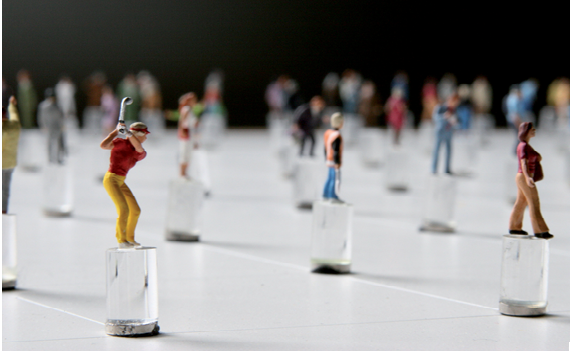
\includegraphics[width=5cm,height=3cm]{img/figurita.png}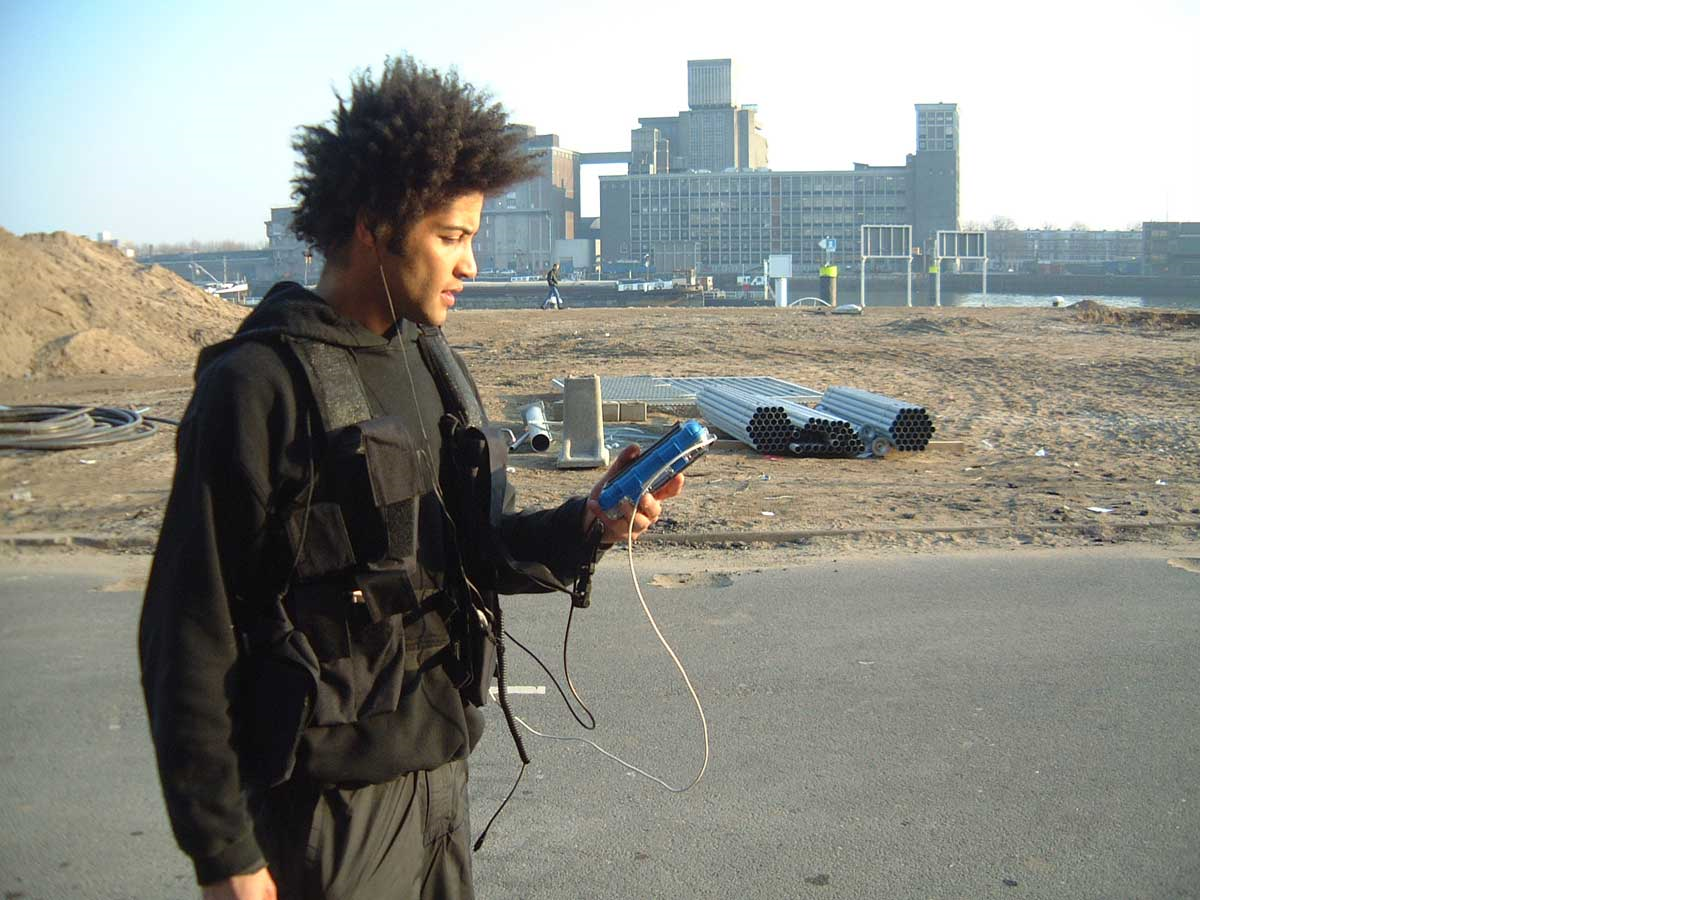
\includegraphics[width=6cm,height=3cm]{img/guy.png}\center
\end{itemize}
\end{frame}

\section{Aplicación móvil para hábitos de lectura usando realidad virtual}
\begin{frame}{Aplicación móvil para hábitos de lectura usando realidad virtual}
\center\textbf{"Diverticuentos"}
\center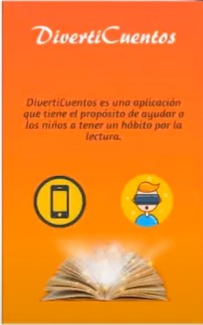
\includegraphics[height=4.5cm]{img/Inicio app movil.jpeg}
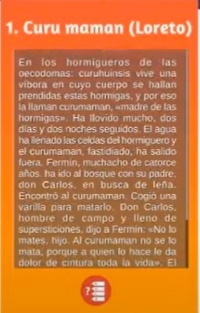
\includegraphics[height=4.5cm]{img/Cuento.jpeg}
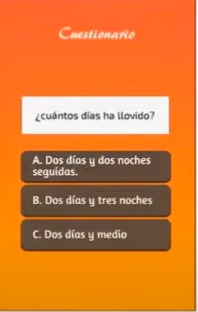
\includegraphics[height=4.5cm]{img/Cuestionario.jpeg}
\end{frame}

\begin{frame}{Lecturas}
\center Se tienen 20 cuentos en 2D y 6 en 3D.
\center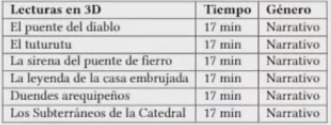
\includegraphics[width=10cm]{img/Cuadro2.jpeg}
\end{frame}

\begin{frame}{Sesiones de aprendizaje}
\center Proceso que considera el ministerio de educación.
\center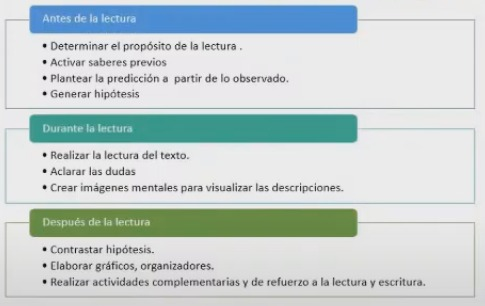
\includegraphics[width=8cm]{img/Sesiones....jpeg}
\end{frame}

\begin{frame}{Resultados}
\center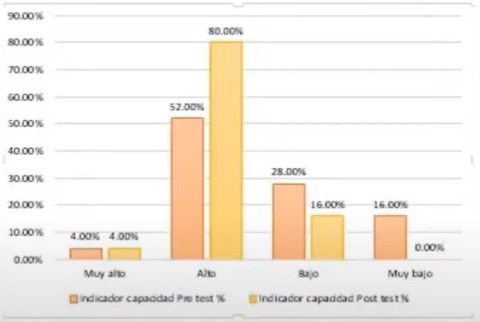
\includegraphics[height=6cm]{img/ResultadosAM.jpeg}
\end{frame}

\begin{frame}{Otras aplicaciones}
\center\textbf{"Unimersiv"}
Historia, el espacio o la anatomía humana.
\center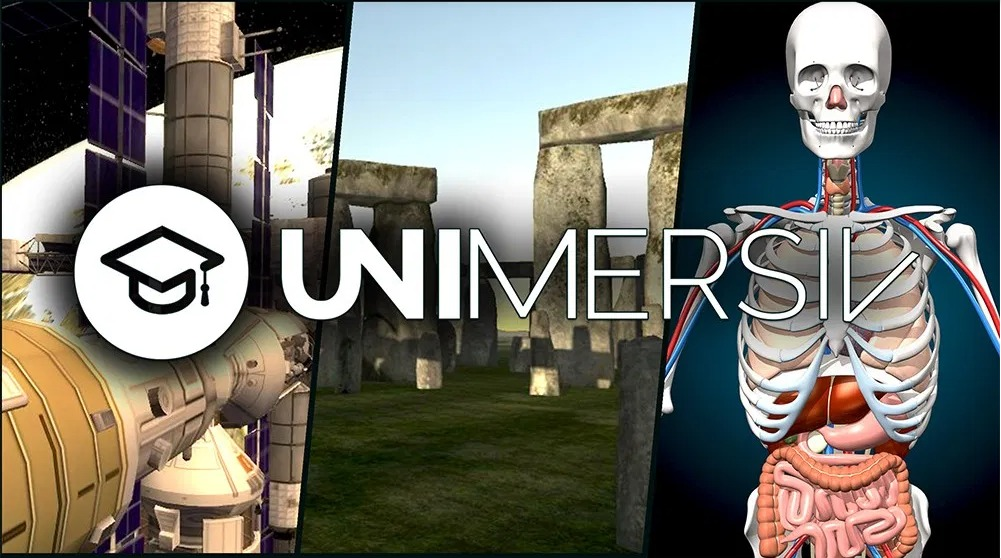
\includegraphics[height= 5cm]{img/unimersiv.jpeg}
\end{frame}

\section{Incremento del Interes de Alumnos en Educación Basica en los Objetos de Aprendizaje Usando Realidad Aumentada en la Geometría}
\begin{frame}
\frametitle{\center Incremento del Interes de Alumnos en Educación Basica en los Objetos de Aprendizaje Usando Realidad Aumentada en la Geometría}
\center 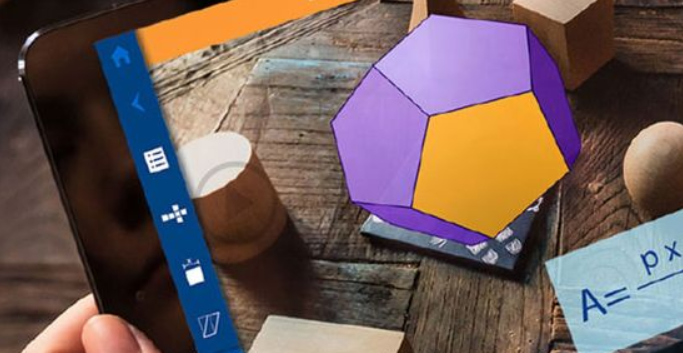
\includegraphics[width=6cm, height=4cm]{img/RA.png} \center
\end{frame}

\begin{frame}
\frametitle{Introducción}
El no poder ver objetos en 3D  hace que los estudiantes tengan que calcular y construir  dichos objetos con métodos tradicionales, en papel (2D) por ejemplo. Esto hace que los problemas sean poco comprendidos y que se perciba la matemática, en especial la geometría, como una materia complicada y hasta muchas veces aburrida produciendo un clima de desmotivación que se ve reflejado en  los resultados de aprendizaje.

\end{frame}

\begin{frame}
\frametitle{Realidad Aumentada}

Azuma (1997) afirma que es un conjunto de tecnologías que permite al usuario ver el mundo real, con objetos virtuales superpuestos o compuestos por el mundo real. Otra definición más actual es la que da Prendes (2015) quien define que la Realidad Aumentada (RA) es una tecnología que superpone a una imagen real obtenida a través de una pantalla imágenes, modelos 3D u otro tipo de informaciones generados por ordenador.

Por lo tanto, la RA complementa la realidad, en lugar de desplazarla por completo.

\textbf{}

\textbf{Caracteristicas:}

\begin{itemize}
\item Combina lo real y lo virtual
\item Interactiva y en tiempo real
\item Registrada en 3D.
\end{itemize}
\end{frame}

\begin{frame}{Metodologia}

Para la realizacion de nuestro objeto de aprendizaje, principalmente se eligió el área de matematicas, después se determino el nivel el cual se decicidio ue fuera 3er grado de primaria y se delimito el tema a "figuras y cuerpos geométricos".

El siguiente paso fue buscar la herramienta adecuada para el modelado 3D para crear los cuerpos geométricos que serian usados en la RA, que después de investigar y probar algunas como 3D Max y Blender, se optó por ser una herramienta sencilla y fácil de manejar.

Finalmente se utilizó el software Aumentaty Author el cual proporciona las etiquetas necesarias y permite unirlas a un modelo de 3D.
\end{frame}

\begin{frame}
\frametitle{}
\center 
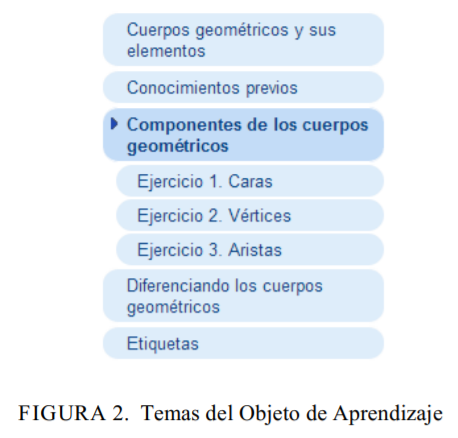
\includegraphics[width=6cm, height=4cm]{img/imagen2.png}
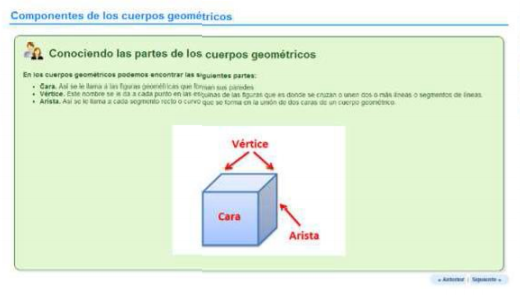
\includegraphics[width=6cm, height=4cm]{img/imagen3.png}

\end{frame}

\begin{frame}
\center 
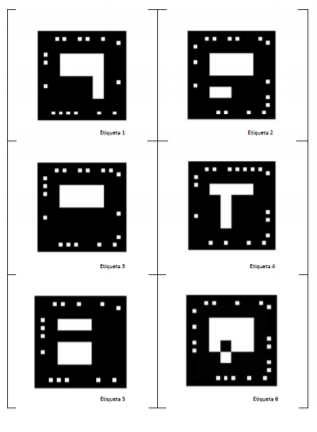
\includegraphics[width=6cm, height=4cm]{img/imagen4.png}
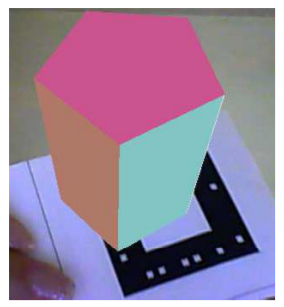
\includegraphics[width=6cm, height=4cm]{img/imagen5.png}

\end{frame}

\begin{frame}
\frametitle{Resultados}
\begin{itemize}
\item Aumento del interes de los alumnos
\item Enseñanza atractiva e interesante
\item Mejora del aprendizaje
\end{itemize}

\end{frame}

\begin{frame}{Conclusiones}
La Realidad aumentada es una tecnologia donde algunas de sus características es que debe ser inmersiva, presencial e interactiva, esta ultima es la razon por la cual se propone como una herramienta util para mejorar el aprendizaje de los alumnos.

Esta tegnologia nos sirve como una herramienta de apoyo para la enseñanza tradicional, mas no sirve como alternativa para esta misma.
\end{frame}


\section{Aplicación de la RA en la enseñanza de Anatomia}
\begin{frame}
\frametitle{Aplicación de la RA en la enseñanza de Anatomia}
\center Human Body AR : Una aplicacion movil para enseñar anatomia a estudiantes utilizando realidad aumentada
\center
\begin{itemize}
\end{itemize}
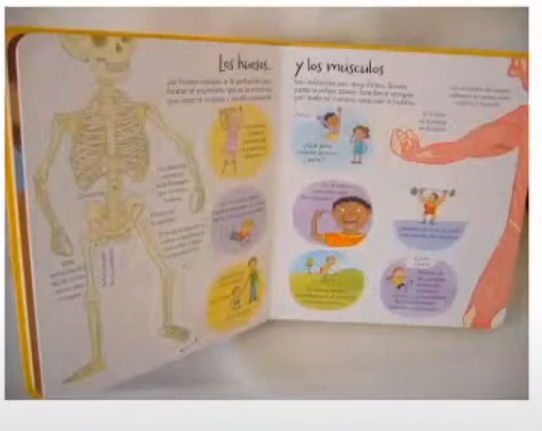
\includegraphics[width=4cm, height=4cm]{img/anatomia.png}
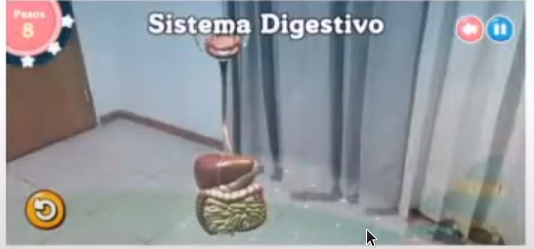
\includegraphics[width=4cm, height=4cm]{img/sistema_digestivo.png}
\end{frame}

\section{Aplicación de la RA en la enseñanza de Anatomia}
\begin{frame}
\frametitle{Aplicación de la RA en la enseñanza de Anatomia}
\center Human Body AR : una aplicacion movil para enseñar anatonima a estudiantes utilizando realidad aumentada
\center
\begin{itemize}
\item La investigacion se centra en el caso de estudio de una aplicacion de realidad aumentada que enseña anatomia teniendo en cuenta la usabilidad educativa.
\end{itemize}
\end{frame}


\begin{frame}
\frametitle{Aplicación de la RA en la enseñanza de Anatomia}
\center Caracteristicas : 
\center
\begin{itemize}
\item Caracteristicas de los organos del cuerpo
\item Funcionamiento de los organos del cuerpo humano
\item Identificar los sistemas del cuerpo humano
\end{itemize}
\end{frame}



\begin{frame}
\frametitle{Aplicación de la RA en la enseñanza de Anatomia}
\center Propuesta : 
\center
\begin{itemize}
\end{itemize}
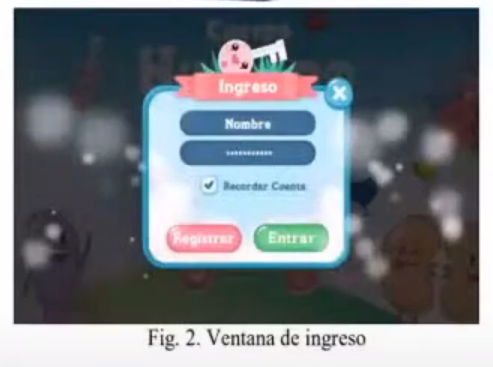
\includegraphics[width=4cm, height=4cm]{img/ingreso.png}
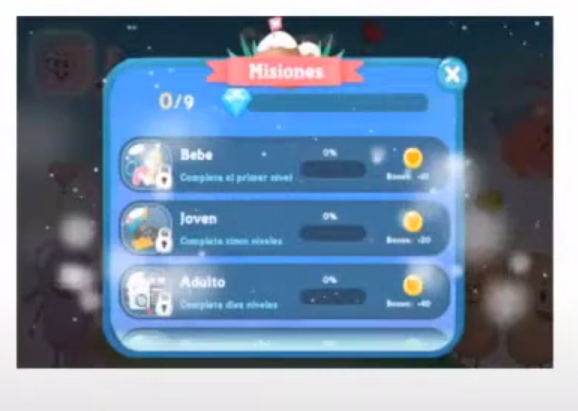
\includegraphics[width=4cm, height=4cm]{img/misiones.png}
\end{frame}


\begin{frame}
\frametitle{Aplicación de la RA en la enseñanza de Anatomia}
\center Propuesta : 
\center
\begin{itemize}
\end{itemize}
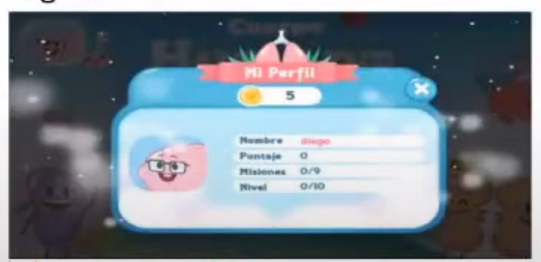
\includegraphics[width=4cm, height=4cm]{img/perfil.png}
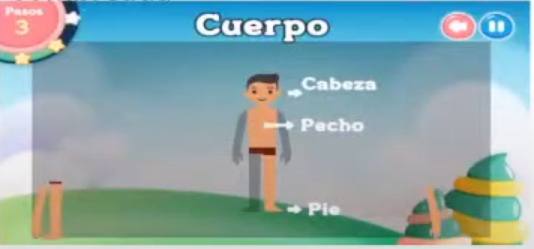
\includegraphics[width=4cm, height=4cm]{img/cuerpo.png}
\end{frame}



\begin{frame}
\frametitle{Aplicación de la RA en la enseñanza de Anatomia}
\center Propuesta : 
\center
\begin{itemize}
\end{itemize}
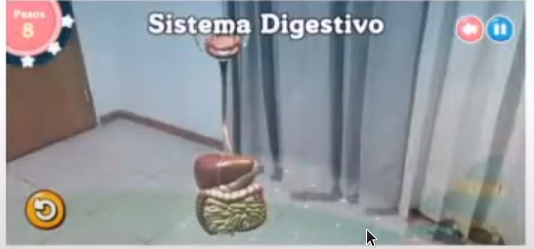
\includegraphics[width=7cm, height=4cm]{img/sistema_digestivo.png}
\end{frame}

\begin{frame}
\frametitle{Aplicación de la RA en la enseñanza de Anatomia}
\center Metodologia y resultados : 
\begin{itemize}
\item las pruebas se realizaron a 20 niños de 5 años y se observaron las acciones y actitudes con ayuda del maestro.
\item Para poder desarrollar una propuesta de heuristicas basadas en Nielsen pero enfocadas en aplicaciones con realidad aumentada, se siguio la metodologia de Rusu quien define gradualmente una serie de seis etapas para establecer nuevas heuristicas de usabilidad.
\item Etapa Exploratoria, descriptiva, correlacional, explicativa de validacion y etapada de refinamiento.
\item De las 20 evaluaciones 16 obtuvieron el valor "Bueno". Es decir no se obtuvo una satisfaccion total, por esto se propuso mejoras en las heuristicas que tuvieron menos puntuacion : Minimizar la carga de memoria, Prevencion de errores, Facilidad de uso, Ayuda y Documentacion.
\end{itemize}
\end{frame}


\begin{frame}
\frametitle{Aplicación de la RA en la enseñanza de Anatomia }
\center Realidad Aumentada aplicada a la
enseñanza de Ciencias Naturales : 
\center
\begin{itemize}
\item En este trabajo se muestran los resultados de una experiencia de extensión desarrollada en el año 2014, donde se utiliza la tecnología Realidad Aumentada para la enseñanza de temas abarcados en Ciencias Naturales en el nivel primario.
\end{itemize}
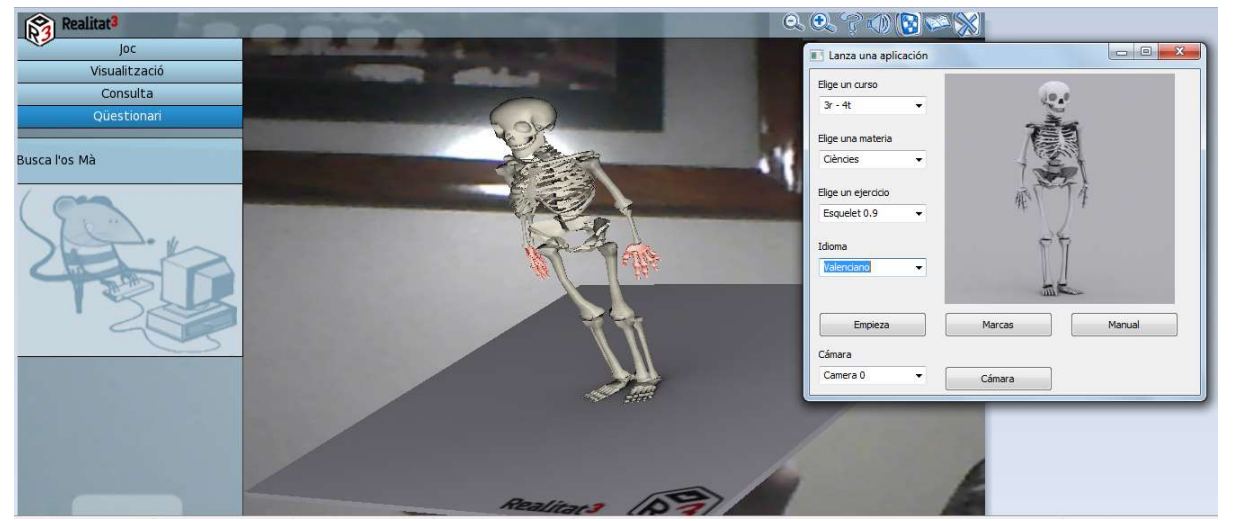
\includegraphics[width=7cm, height=4cm]{img/sistema_oseo.png}
\end{frame}


\begin{frame}
\frametitle{Aplicación de la RA en la enseñanza de Anatomia}
\center Herramientas utilizadas ONLINE  : 
\center
\begin{itemize}
\item Anatomía: si bien es agradable a la vista no es demasiado intuitiva, por ejemplo el marcador puede encontrarse bajo un botón rotulado download que no identifica adecuadamente que es lo que se está descargando. http://www.ediamsistemas.com/anatomia/ 
\item LearnAR: es simple y se explican
claramente los pasos a seguir para poder utilizarla. Además se explica claramente desde donde deben descargarse los marcadores. http://www.learnar.org/ 
\end{itemize}
\end{frame}


\begin{frame}
\frametitle{Aplicación de la RA en la enseñanza de Anatomia}
\center Herramientas utilizadas OFFLINE para PC : 
\center
\begin{itemize}
\item Corinth Anatomy: es simple de usar e intuitiva.
\item Aumentaty Autor: es simple de usar e intuitiva.
\item BuildAr : es simple de usar e intuitiva. 
\end{itemize}
\end{frame}

\begin{frame}
\frametitle{Aplicación de la RA en la enseñanza de Anatomia}
\center Imagenes : 
\begin{itemize}
\end{itemize}
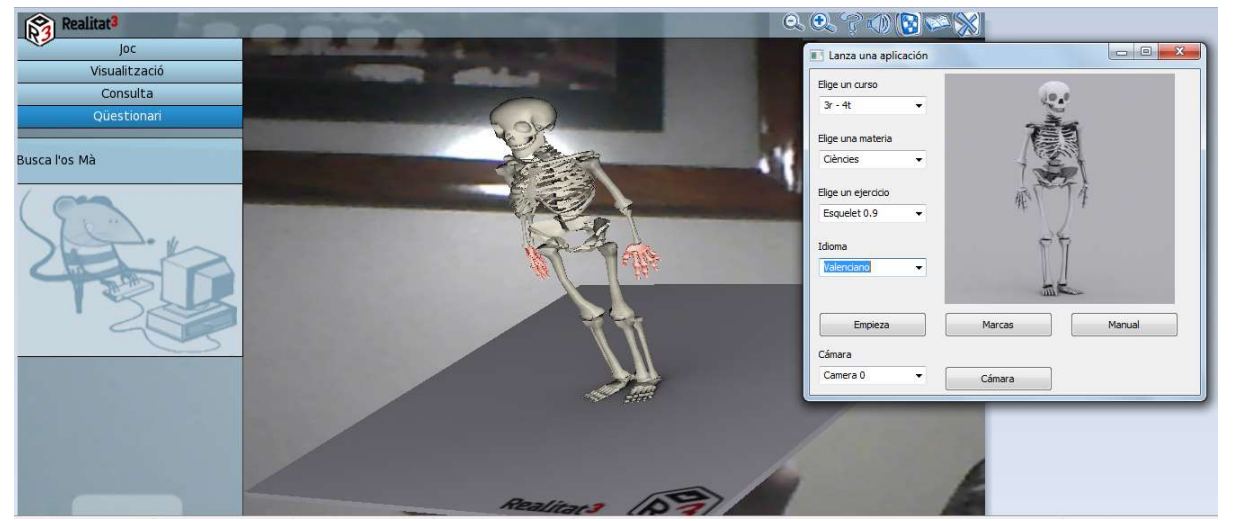
\includegraphics[width=7cm, height=4cm]{img/sistema_oseo.png}
\end{frame}

\begin{frame}
\frametitle{Aplicación de la RA en la enseñanza de Anatomia}
\center Imagenes : 
\begin{itemize}
\end{itemize}
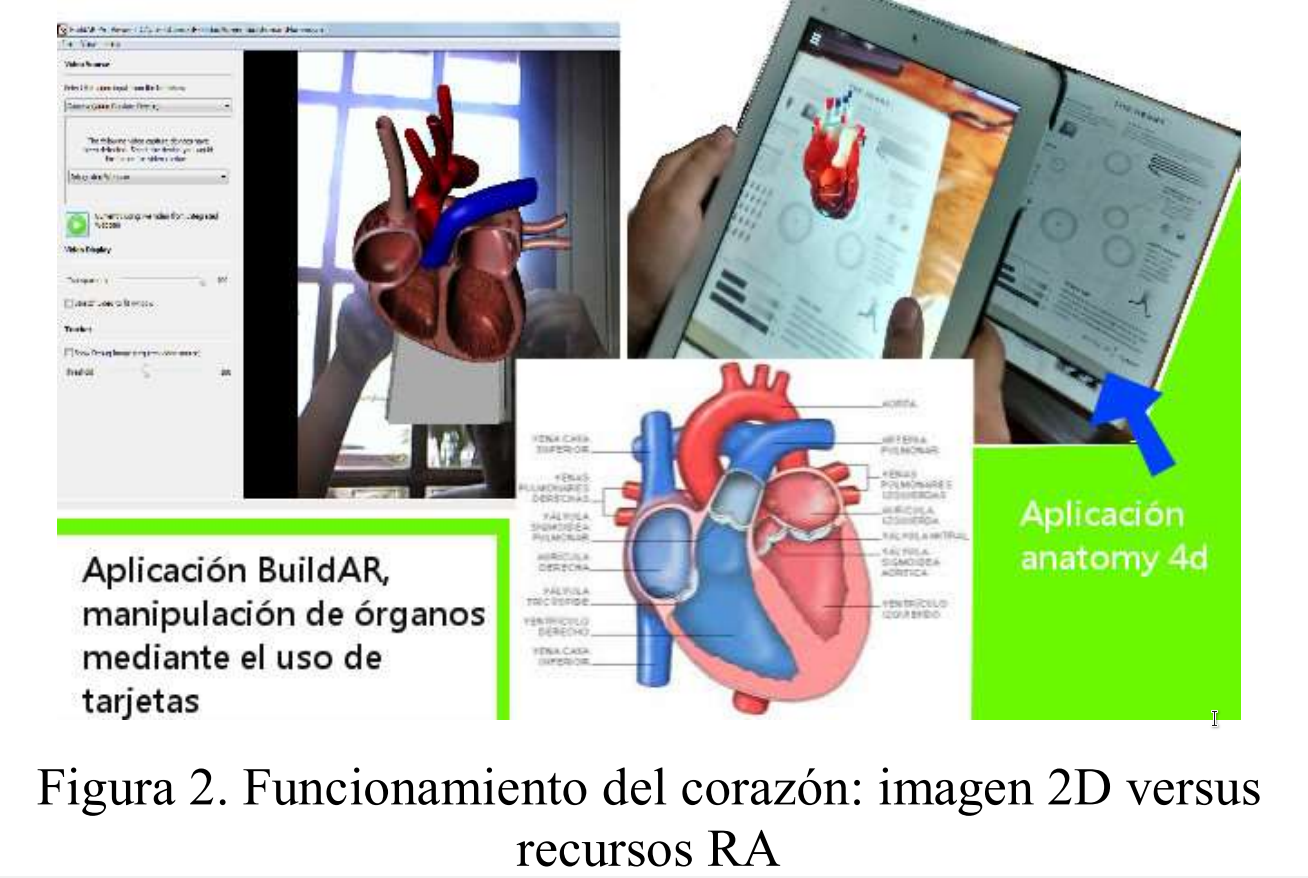
\includegraphics[width=7cm, height=4cm]{img/comparacion.png}
\end{frame}

\begin{frame}
\frametitle{Aplicación de la RA en la enseñanza de Anatomia}
\center Imagenes : 
\begin{itemize}
\end{itemize}
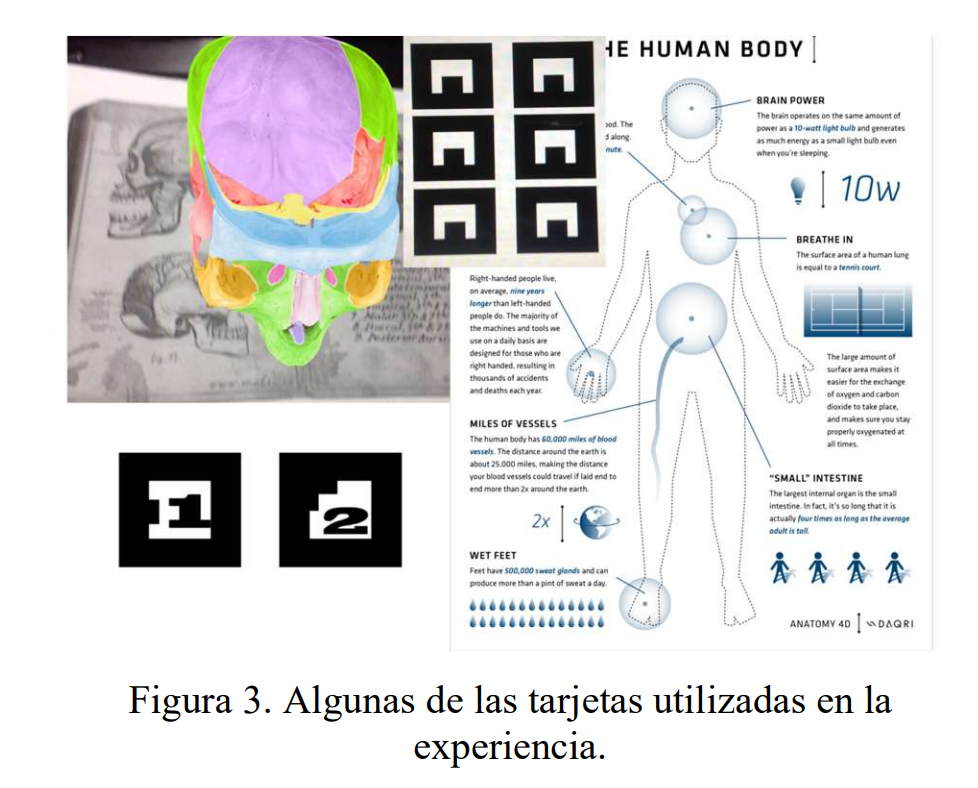
\includegraphics[width=7cm, height=4cm]{img/tarjeta.png}
\end{frame}


\begin{frame}
\frametitle{Aplicación de la RA en la enseñanza de Anatomia}
\center Resultados y trabajos a futuro : 
\begin{itemize}
\item Resultados : Sólo 2 niños del grupo manifestaron conocer la Realidad
Aumentada, aunque no la habían probado. Y a simple vista fue
evidente el entusiasmo que presentaron los niños ante los
recursos de RA trabajados.
\item Trabajos a futuro : Se espera extraer una serie de rutinas/patrones pedagógicos de diseño
y la puesta en práctica de actividades que incorporen
recursos empleando la tecnología de Realidad Aumentada
en contextos de Educación universitaria. 
\end{itemize}
\end{frame}




\section{Referencias}
%References frame
\begin{frame}
\frametitle{Referencias}
\begin{itemize}
\item Fracchia, C. C., Alonso de Armiño, A. C., and Martins, A. (2015). Realidad Aumentada aplicada a la enseñanza de Ciencias Naturales.TE  and   ET.
\item Escartín, E. (s/f). La realidad virtual, una tecnología educativa a nuestro alcance. Instituto Superior Politécnico “José A. Echeverría”.
ISPJAE (Cuba)
\item Sánchez, L. (2014). Juegos pervasivos: el potencial ubicuo de los dispositivos móviles. ESNE Escuela Universitaria de Diseño, Innovación y Tecnología
\item Azuma, R. T. (1997). A survey of augmented reality. Presence: Teleoperators & Virtual Environments, 6(4), 355-385.
\item Prendes Espinosa, C. (2015). Realidad aumentada y educación: análisis de experiencias prácticas. Píxel-Bit. Revista de Medios y Educación, 46, 187-203.
\end{itemize}
\end{frame}
\end{document}
